%%%%%%%%%%%%%%%%%%%%%%%%%%%%%%%%%%%%%%%%%%%%%%%%%%%%%%%%%%%%%%%%%%%%%%%%

%%% LaTeX Template for ECAI Papers 
%%% Prepared by Ulle Endriss (version 1.0 of 2023-12-10)

%%% To be used with the ECAI class file ecai.cls.
%%% You also will need a bibliography file (such as mybibfile.bib).

%%%%%%%%%%%%%%%%%%%%%%%%%%%%%%%%%%%%%%%%%%%%%%%%%%%%%%%%%%%%%%%%%%%%%%%%

%%% Start your document with the \documentclass{} command.
%%% Use the first variant for the camera-ready paper.
%%% Use the second variant for submission (for double-blind reviewing).

\documentclass{ecai} 
%\documentclass[doubleblind]{ecai} 

%%%%%%%%%%%%%%%%%%%%%%%%%%%%%%%%%%%%%%%%%%%%%%%%%%%%%%%%%%%%%%%%%%%%%%%%

%%% Load any packages you require here. 

\usepackage{latexsym}
\usepackage{amssymb}
\usepackage{amsmath}
\usepackage{amsthm}
\usepackage{booktabs}
\usepackage{enumitem}
\usepackage{graphicx}
\usepackage{adjustbox}
\usepackage{color}
\usepackage{placeins}
\usepackage{float}
\usepackage{caption}

%%%%%%%%%%%%%%%%%%%%%%%%%%%%%%%%%%%%%%%%%%%%%%%%%%%%%%%%%%%%%%%%%%%%%%%%

%%% Define any theorem-like environments you require here.

\newtheorem{theorem}{Theorem}
\newtheorem{lemma}[theorem]{Lemma}
\newtheorem{corollary}[theorem]{Corollary}
\newtheorem{proposition}[theorem]{Proposition}
\newtheorem{fact}[theorem]{Fact}
\newtheorem{definition}{Definition}

%%%%%%%%%%%%%%%%%%%%%%%%%%%%%%%%%%%%%%%%%%%%%%%%%%%%%%%%%%%%%%%%%%%%%%%%

%%% Define any new commands you require here.

\newcommand{\BibTeX}{B\kern-.05em{\sc i\kern-.025em b}\kern-.08em\TeX}

%%%%%%%%%%%%%%%%%%%%%%%%%%%%%%%%%%%%%%%%%%%%%%%%%%%%%%%%%%%%%%%%%%%%%%%%

\begin{document}

%%%%%%%%%%%%%%%%%%%%%%%%%%%%%%%%%%%%%%%%%%%%%%%%%%%%%%%%%%%%%%%%%%%%%%%%

\begin{frontmatter}

%%% Use this command to specify your submission number.
%%% In doubleblind mode, it will be printed on the first page.

\paperid{123} 

%%% Use this command to specify the title of your paper.

\title{LLM-Augmented Optimization for Singapore Travel Itinerary Planning}

%%% Use this combinations of commands to specify all authors of your 
%%% paper. Use \fnms{} and \snm{} to indicate everyone's first names 
%%% and surname. This will help the publisher with indexing the 
%%% proceedings. Please use a reasonable approximation in case your 
%%% name does not neatly split into "first names" and "surname".
%%% Specifying your ORCID digital identifier is optional. 
%%% Use the \thanks{} command to indicate one or more corresponding 
%%% authors and their email address(es). If so desired, you can specify
%%% author contributions using the \footnote{} command.

\author[A]
{\fnms{Daniel}~\snm{James}}

\author[A]
{\fnms{Leonardo}}

\author[A]
{\fnms{Jing Shen}~\snm{Tai}}

\author[A]
{\fnms{Valerian}~\snm{Yap}}

\author[A]
{\fnms{Hoong Chuin}~\snm{Lau}\thanks{Corresponding Author. Email: hclau@smu.edu.sg.}}

\address[A]{School of Computing and Information Systems, Singapore Management University}

%%% Use this environment to include an abstract of your paper.

\begin{abstract}
We present a hybrid approach combining Large Language Models (LLMs) and Operations Research to generate travel itineraries for Singapore. Recognizing that traveler preferences vary across demographics, our system produces personalized plans that balance cost, travel time, and satisfaction. LLM agents interpret natural language preferences and convert them into structured variables, which are then optimized using Adaptive Large Neighborhood Search. Our contribution lies in bridging natural language inputs with combinatorial optimization to produce feasible, context-aware itineraries through the use of multi-agents. A distinguishing feature is the incorporation of meals in hawker centers. We benchmark our system against LLM-only and optimization-only baselines to demonstrate that it significantly improves personalized user objectives. 
\end{abstract}

\end{frontmatter}

% adjust spacing between items
\setlist[itemize]{topsep=-1pt, partopsep=-1pt, parsep=-1pt, itemsep=0pt}
\setlist[enumerate]{topsep=-1pt, partopsep=-1pt, parsep=-1pt, itemsep=0pt}

\raggedbottom  % Allow page bottom flexibility

%%%%%%%%%%%%%%%%%%%%%%%%%%%%%%%%%%%%%%%%%%%%%%%%%%%%%%%%%%%%%%%%%%%%%%%%

\section{Introduction}
Our goal is to develop a personalized travel itinerary planner demo product for tourists visiting Singapore, capable of allowing natural language inputs and predefined fields to generate a feasible yet personalized itinerary by minimizing travel cost, minimizing total transit time between locations, and maximizing satisfaction that aligns with persona-specific preferences. 

Our commercial inspiration was primarily drawn from Pelago by Singapore Airlines, an AI-powered trip planner platform that covers over 2,000 destinations (Pelago, 2025). While Pelago appears to be employing an LLM-based recommendation engine, our work diverges by introducing a multi-agent LLM system that is combined with Operation Research (OR) optimization techniques.

In this paper, we propose My Travel Itinerary Buddy – Automatic Itinerary (MITB–AI). Our goal is to explore the following questions: 
\begin{enumerate}
    \item Recognising the hallucination in LLM, to what extent can LLM alone generate realistic and feasible travel itineraries? 
    \item Assuming we have an LLM agent (e.g. a domain-expert in Singapore attractions, equipped with memory, knowledge base and tools), can it handle reasoning consistency and personalisation without hallucinating? What is the trade-off for having multiple domain experts in our system?
    \item What are the quantitative and qualitative trade-offs between optimization-only, LLM-only, multi-agent and hybrid optimization itinerary planning pipelines?
\end{enumerate}

MITB-AI is geographically and thematically scoped to the context of Singapore's deep local culture. 
Specifically, Singapore's Hawker Culture was listed as one of UNESCO's Representative List of the Intangible Cultural Heritage of Humanity in 2020. Hawker centers (HC) are places where Singaporeans from all walks of life gather. Most travel apps ignore the aspect of incorporating meals in HCs, allowing tourists not only to enjoy the rich food culture but, more importantly, to experience the ambience of daily life of Singapore in such a setting. 
Hence, our system focuses on two categories of points of interest (POIs): (i) attractions, and (ii) hawker centers. In total, our curated dataset includes over 85 unique POIs and was inspired by research papers for optimizing travel itineraries with AI algorithm (Barua et al, 2024), TRIP-PAL (JP Morgan AI Research, 2024).

%%%%%%%%%%%%%%%%%%%%%%%%%%%%%%%%%%%%%%%%%%%%%%%%%%%%%gm%%%%%%%%%%%%%%%%%%%
\section{Innovation and Technical Contribution}
\subsection{LLM and Multi-Agent Framework}
MITB-AI brings together LLM flexibility and OR rigor in solving real-world planning problems.
While LLMs excel at interpreting and generating human-like text, they remain passive systems—limited to single-turn interactions and lacking memory. This poses challenges for travel itinerary planning, which requires structured decision-making, external data retrieval (e.g., attraction costs, ratings), and multi-step context tracking. Passive LLMs may generate generic itineraries but fall short on personalized requests like “prefer scenic routes” or “maximize shopping time within budget.”

To overcome this, we transform LLMs into autonomous agents equipped with tool-calling (e.g., Google Maps APIs), memory for goal retention, and Retrieval Augmented Generation (RAG) to incorporate external knowledge. This shifts the LLM from a reactive responder to a goal-directed planner. Our Agentic RAG framework enriches itineraries with contextual data such as attraction hours and hawker durations.

Although a single agent could manage the full pipeline, monolithic setups often underperforms in domain-specific reasoning. We therefore adopt a multi-agent architecture, assigning distinct tasks—such as attraction filtering or optimization translation—to specialized agents for better performance and modularity and even incorporating a feasibility checker for the itinerary that was updated due to modification of preference by the user.

\subsection{Adaptive Large Neighborhood Search (ALNS)}
ALNS is an optimization technique that offers greater flexibility in navigating complex, dynamic solution spaces. In our demo, ALNS proved most effective in handling the multi-objective nature and constraints of itinerary planning. Inspired by the modified ALNS for Family Tourist Route Planning (Khamsing, 2021), our destroy and repair operators modify parts of the itinerary by replacing POIs based on high-quality input from the multi-agentic workflow. 

\FloatBarrier
\begin{figure*}[h]
    \centering
    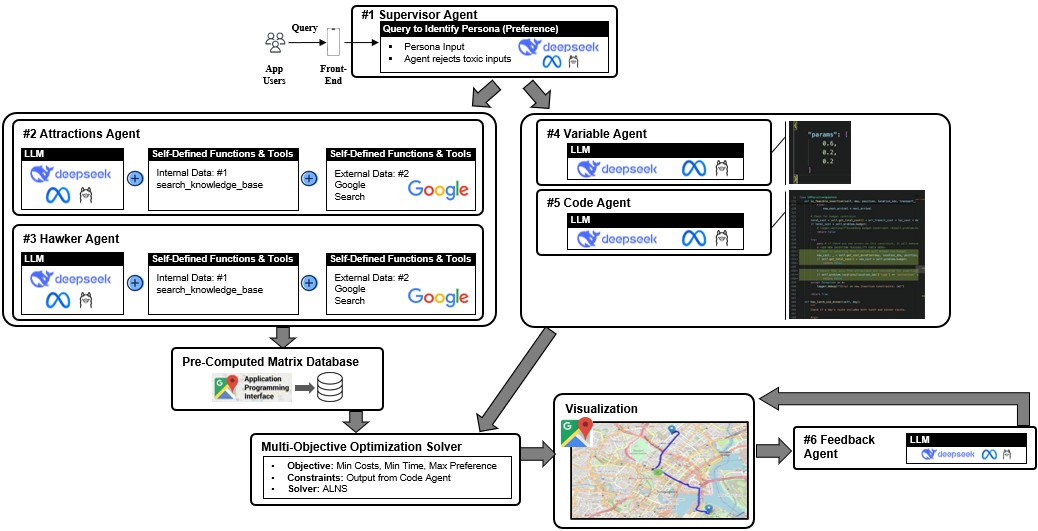
\includegraphics[width=0.75\linewidth]{MITB AI Architecture Image.jpg}
    \caption{Multi-Agent Architecture (MITB-AI)}
    \label{fig:Workflow Diagram}
\end{figure*}
    
\section{System Overview}
The MITB-AI system adopts a modular multi-agent architecture to support the generation of realistic, multi-objective travel itineraries based on user preferences. Each agent is specialized to handle a distinct sub-task in the overall pipeline, enabling more scalable, interpretable, and error-resilient behavior than monolithic LLM agents.

Figure~\ref{fig:Workflow Diagram} illustrates the system architecture. The \textbf{Supervisor Agent} manages user input routing and intent classification, while filtering out harmful or nonsensical requests. Downstream agents include the \textbf{Attractions Agent} and \textbf{Hawker Agent}, which perform semantic retrieval on user queries to match relevant POIs from a PostgreSQL-hosted database enriched with metadata such as geolocation, ratings, and opening hours. The \textbf{Variable Agent} translates a user’s persona into optimization weights (e.g., prioritizing cost vs. satisfaction), and the \textbf{Code Agent} transforms free-text constraints into structured logic for optimization. The \textbf{Feedback Agent} supports mid-session itinerary adjustments when the user modifies constraints or preferences.

The system incorporates an ALNS algorithm once user preferences have been translated into structured variables and constraints. The tool is used to generate an initial itinerary that balances travel cost, duration, and satisfaction. The optimization is performed only once during the initial planning phase and operates on a precomputed route matrix generated from Google Maps API data. The details of the ALNS operators are discussed in Section 3.2.

On the user interface, the system supports both natural language input and structured form-based input. The output consists of a personalized day-by-day itinerary that includes POIs, mealtimes, estimated travel times, and cost estimates. These are rendered both as textual summaries and visual map in Streamlit.

\section{Problem Definition}
The goal of MITB-AI is to generate multi-day travel itinerary for a tourist visiting Singapore, consisting of a sequence of POIs – including both attractions and HCs. This is subject to user-defined constraints (e.g. budget, number of days and person types) while optimizing for the following objectives: (1) minimize costs, (2) minimize travel time, and (3) maximize traveler’s satisfaction. This problem can be classified as a multi-objective optimization task, where the system must select and order POIs over multiple days while satisfying both hard and soft constraints (Fan, et al., 2024).

\subsection{Assumptions}
The assumptions that we have incorporated in our itinerary planners includes: 
\begin{itemize}
    \item all POIs are open from 9:00 AM to 10:00 PM.
    \item travelers return to the same hotel by the end of the day.
\end{itemize}
\vspace{-0.1cm}

\subsection{Route Matrix Generation using Google Maps API}
To support accurate travel time estimation between POIs, we constructed a route matrix using Google Maps API.

\section{Demonstration Scenarios}
We evaluated the hybrid LLM-augmented optimization system using various personas of travelers and preferences representative of typical visitors to Singapore. Each experimental scenario began as a natural language request parsed by our multi-agent LLM into structured itinerary parameters, capturing traveler preferences such as budget, attractions, food types, and transportation modes.
For instance, one scenario involved a Family Tourist persona visiting for three days with a modest budget, seeking family-friendly attractions and affordable local dining options. Another featured a Cultural Enthusiast interested in exploring heritage sites and authentic hawker food experiences.
An essential capability demonstrated was the system’s ability to dynamically adjust itineraries in response to real-time changes. For example, during the testing, the Nature Lover persona initially received an itinerary prioritizing outdoor activities. When a simulated weather event was introduced—rainy conditions—the system promptly updated the itinerary upon the user's request to substitute indoor attractions or sheltered natural spots, ensuring a seamless travel experience despite disruptions. 
Key demonstrated functionalities included:
\begin{itemize}
    \item \textbf{Dynamic Updates}: Real-time itinerary adjustments in response to unexpected conditions, such as adverse weather or closures.
    \item \textbf{Multi-objective Optimization}: Balance cost, travel duration, and visitor satisfaction.
    \item \textbf{Explicit Time-window Constraints}: Performing accurate meal schedules.
    \item \textbf{Transportation Selection}: Options between public transportation and driving modes.
    \item \textbf{Detailed Itinerary Outputs}: Comprehensive itineraries detailing routes, costs, timings, and satisfaction metrics.
\end{itemize}
This demonstration underscored the flexibility and responsiveness of the system in producing optimized, feasible, and adaptable travel itineraries tailored to changing visitor needs.

\section{Deployment / Impact / Maturity}
% - deployment status
% - real users and stakeholders
% - performance metrics and evaluations
% \textbf{!!! try to use \url{https://arxiv.org/pdf/2402.01622} for the benchmark}
MITB-AI has been implemented as a fully functional prototype using a containerized backend architecture with Docker, PostgreSQL for metadata storage, and APIs for LLM agent execution and Google Maps integration. The system supports real-time itinerary generation and dynamic updates, and has been tested with a representative set of user personas. In experimental comparisons, we evaluate three variants: (i) a vanilla multi-agent LLM planner, (ii) the same planner enhanced with ALNS optimization, and (iii) an extended version incorporating a custom tool function to handle dynamic user inputs. Across these scenarios, the ALNS-enhanced model consistently produces more feasible and satisfying itineraries, demonstrating the effectiveness of our hybrid approach. System response times remain within 5 seconds even under moderate load, and the modular design ensures that additional agents or logic layers can be integrated as the product scales. These results suggest a strong potential for real-world deployment in travel planning platforms targeting both individual users and tourism service providers. 
\vspace{-0.1cm}

% still interesting, but need to go when we don't have space
% if cannot fit, can show in video, to demonstrate rigor of our experiment
% Result from Vanilla ALNS is the least important bit of this paper, because this is not an optimization paper
\begin{table}[htbp]
    \centering
    \begin{adjustbox}{width=0.48\textwidth} % THIS IS SO SMALL THO?
    \begin{tabular}{|c|c|c|c|c|c|c|c|c|c|c|c|}
         \hline
         \multicolumn{3}{|c|}{\textbf{Objective Weights}} & \multicolumn{2}{c|}{\textbf{Expense (SGD)}} & \multicolumn{2}{c|}{\textbf{Travel Time (m)}} & \multicolumn{2}{c|}{\textbf{Satisfaction}} & \multicolumn{2}{c|}{\textbf{Objective Value}} & \textbf{Runtime (s)} \\
         \hline
         \textbf{Budget} & \textbf{Travel Time} & \textbf{Satisfaction} & \textbf{Initial} & \textbf{ALNS} & \textbf{Initial} & \textbf{ALNS} & \textbf{Initial} & \textbf{ALNS} & \textbf{Initial} & \textbf{ALNS} & \textbf{ALNS} \\
         \hline
         0.8 & 0.1 & 0.1 & 281.84 & 208.33 & 402 & 478 & 73.2 & 69.7 & 0.27 & 0.2 & 33.95 \\
         0.1 & 0.8 & 0.1 & 281.84 & 256.08 & 402 & 209 & 73.2 & 58.8 & 0.32 & 0.24 & 56.33 \\
         0.1 & 0.1 & 0.8 & 281.84 & 284.79 & 402 & 510 & 73.2 & 80.9 & -0.31 & -0.36 & 36.33 \\
         0.45 & 0.45 & 0.1 & 281.84 & 190.56 & 402 & 109 & 73.2 & 42 & 0.55 & 0.4 & 68.43 \\
         0.1 & 0.45 & 0.45 & 281.84 & 290.04 & 402 & 228 & 73.2 & 70.7 & -0.07 & -0.11 & 81.04 \\
         0.45 & 0.1 & 0.45 & 281.84 & 217.49 & 402 & 643 & 73.2 & 71.6 & 0.1 & 0.03 & 46.3 \\
         0.33 & 0.33 & 0.33 & 281.84 & 221.48 & 402 & 188 & 73.2 & 59.1 & 0.19 & 0.13 & 50.95 \\
         \hline
    \end{tabular}
    \end{adjustbox}
    \caption{Results from vanilla ALNS}
\end{table}
\vspace{-0.3cm}

\begin{table}[htbp]
    \centering
    \begin{adjustbox}{width=0.48\textwidth}
    \begin{tabular}{|c|c|c|c|c|c|c|c|c|c|c|c|}
         \hline
         \multicolumn{3}{|c|}{\textbf{Objective Weights}} & \multicolumn{2}{c|}{\textbf{Expense (SGD)}} & \multicolumn{2}{c|}{\textbf{Travel Time (m)}} & \multicolumn{2}{c|}{\textbf{Satisfaction}} & \multicolumn{2}{c|}{\textbf{Objective Value}} & \textbf{Runtime (s)} \\
         \hline
         \textbf{Budget} & \textbf{Travel Time} & \textbf{Satisfaction} & \textbf{Initial} & \textbf{ALNS} & \textbf{Initial} & \textbf{ALNS} & \textbf{Initial} & \textbf{ALNS} & \textbf{Initial} & \textbf{ALNS} & \textbf{ALNS} \\
         \hline
         0.4 & 0.3 & 0.3 & 275.86 & 198.24 & 303 & 343 & 79 & 79 & 0.22 & 0.14 & 18.53 \\
         0.6 & 0.2 & 0.2 & 100.99 & 104.59 & 837 & 246 & 75 & 69 & 0.38 & 0.33 & 19.86 \\
         0.4 & 0.2 & 0.4 & 176.43 & 120.83 & 491 & 255 & 75 & 79 & -0.01 & -0.15 & 46.93 \\
         0.4 & 0.3 & 0.3 & 264.24 & 348.24 & 287 & 278 & 78 & 88 & 0.13 & 0.1 & 22.62 \\
         0.2 & 0.1 & 0.7 & 193.6 & 194.67 & 861 & 802 & 64 & 74 & -0.24 & -0.32 & 13.69 \\
         0.4 & 0.2 & 0.4 & 186.8 & 178.42 & 937 & 782 & 72 & 80 & 0.04 & -0.03 & 19.43 \\
         0.4 & 0.3 & 0.3 & 234.25 & 328.1 & 288 & 246 & 75 & 89 & 0.1 & 0.07 & 24.44 \\
         0.3 & 0.2 & 0.5 & 140.87 & 148.1 & 529 & 302 & 82 & 84 & -0.14 & -0.18 & 28.74 \\
         0.6 & 0.2 & 0.2 & 152.39 & 112.48 & 725 & 373 & 83 & 89 & 0.44 & 0.31 & 36.92 \\
         0.4 & 0.3 & 0.3 & 181.76 & 154.72 & 567 & 358 & 75 & 81 & 0.2 & 0.14 & 59.95 \\
         \hline
    \end{tabular}
    \end{adjustbox}
    \caption{Results from ALNS with inputs from traditional LLM}
    \label{tab:my_label}
\end{table}
\vspace{-0.3cm}

\begin{table}[htbp]
    \centering
    \begin{adjustbox}{width=0.48\textwidth}
    \begin{tabular}{|c|c|c|c|c|c|c|c|c|c|c|c|c|}
         \hline
         \multicolumn{3}{|c|}{\textbf{Objective Weights}} & \multicolumn{2}{c|}{\textbf{Expense (SGD)}} & \multicolumn{2}{c|}{\textbf{Travel Time (m)}} & \multicolumn{2}{c|}{\textbf{Satisfaction}} & \multicolumn{2}{c|}{\textbf{Objective Value}} & \multicolumn{2}{c|}{\textbf{Runtime (s)}} \\
         \hline
         \textbf{Budget} & \textbf{Travel Time} & \textbf{Satisfaction} & \textbf{Initial} & \textbf{ALNS} & \textbf{Initial} & \textbf{ALNS} & \textbf{Initial} & \textbf{ALNS} & \textbf{Initial} & \textbf{ALNS} & \textbf{Agentic} & \textbf{ALNS} \\
         \hline
         0.5 & 0.3 & 0.2 & 191.3 & 206.87 & 456 & 346 & 79.7 & 86 & 0.32 & 0.28 & 190.89 & 35.61 \\
         0.6 & 0.2 & 0.2 & 133.28 & 103.77 & 581 & 258 & 79 & 83 & 0.47 & 0.31 & 158.73 & 28.65 \\
         0.5 & 0.3 & 0.2 & 109.37 & 121.78 & 627 & 288 & 76.5 & 85 & 0.35 & 0.27 & 153.47 & 18.01 \\
         0.3 & 0.2 & 0.5 & 248.39 & 394.85 & 560 & 262 & 80.7 & 88 & -0.13 & -0.21 & 265.37 & 72.97 \\
         0.3 & 0.4 & 0.3 & 138.33 & 134.57 & 760 & 536 & 73 & 76.5 & 0.21 & 0.17 & 193.24 & 33.24 \\
         0.3 & 0.2 & 0.5 & 184.23 & 164.2 & 800 & 573 & 64.2 & 62 & 0.06 & 0.02 & 190.28 & 5.01 \\
         0.4 & 0.3 & 0.3 & 188.91 & 187.61 & 496 & 301 & 75.6 & 72.2 & 0.18 & 0.15 & 191.03 & 6.53 \\
         0.3 & 0.2 & 0.5 & 179.46 & 151.71 & 792 & 379 & 71.8 & 78.2 & -0.02 & -0.13 & 157.18 & 28.22 \\
         0.7 & 0.2 & 0.1 & 137.62 & 120 & 828 & 278 & 74 & 81 & 0.58 & 0.47 & 142.5 & 25.95 \\
         0.4 & 0.3 & 0.3 & 180.93 & 168.02 & 615 & 279 & 76.6 & 79.6 & 0.2 & 0.12 & 200.98 & 42.27 \\
         \hline
    \end{tabular}
    \end{adjustbox}
    \caption{Results from ALNS with inputs from Agentic RAG}
    \label{tab:my_label}
    \captionsetup{skip=2pt}
\end{table}
\vspace{-0.3cm}

\begin{figure}[H]
    \centering
    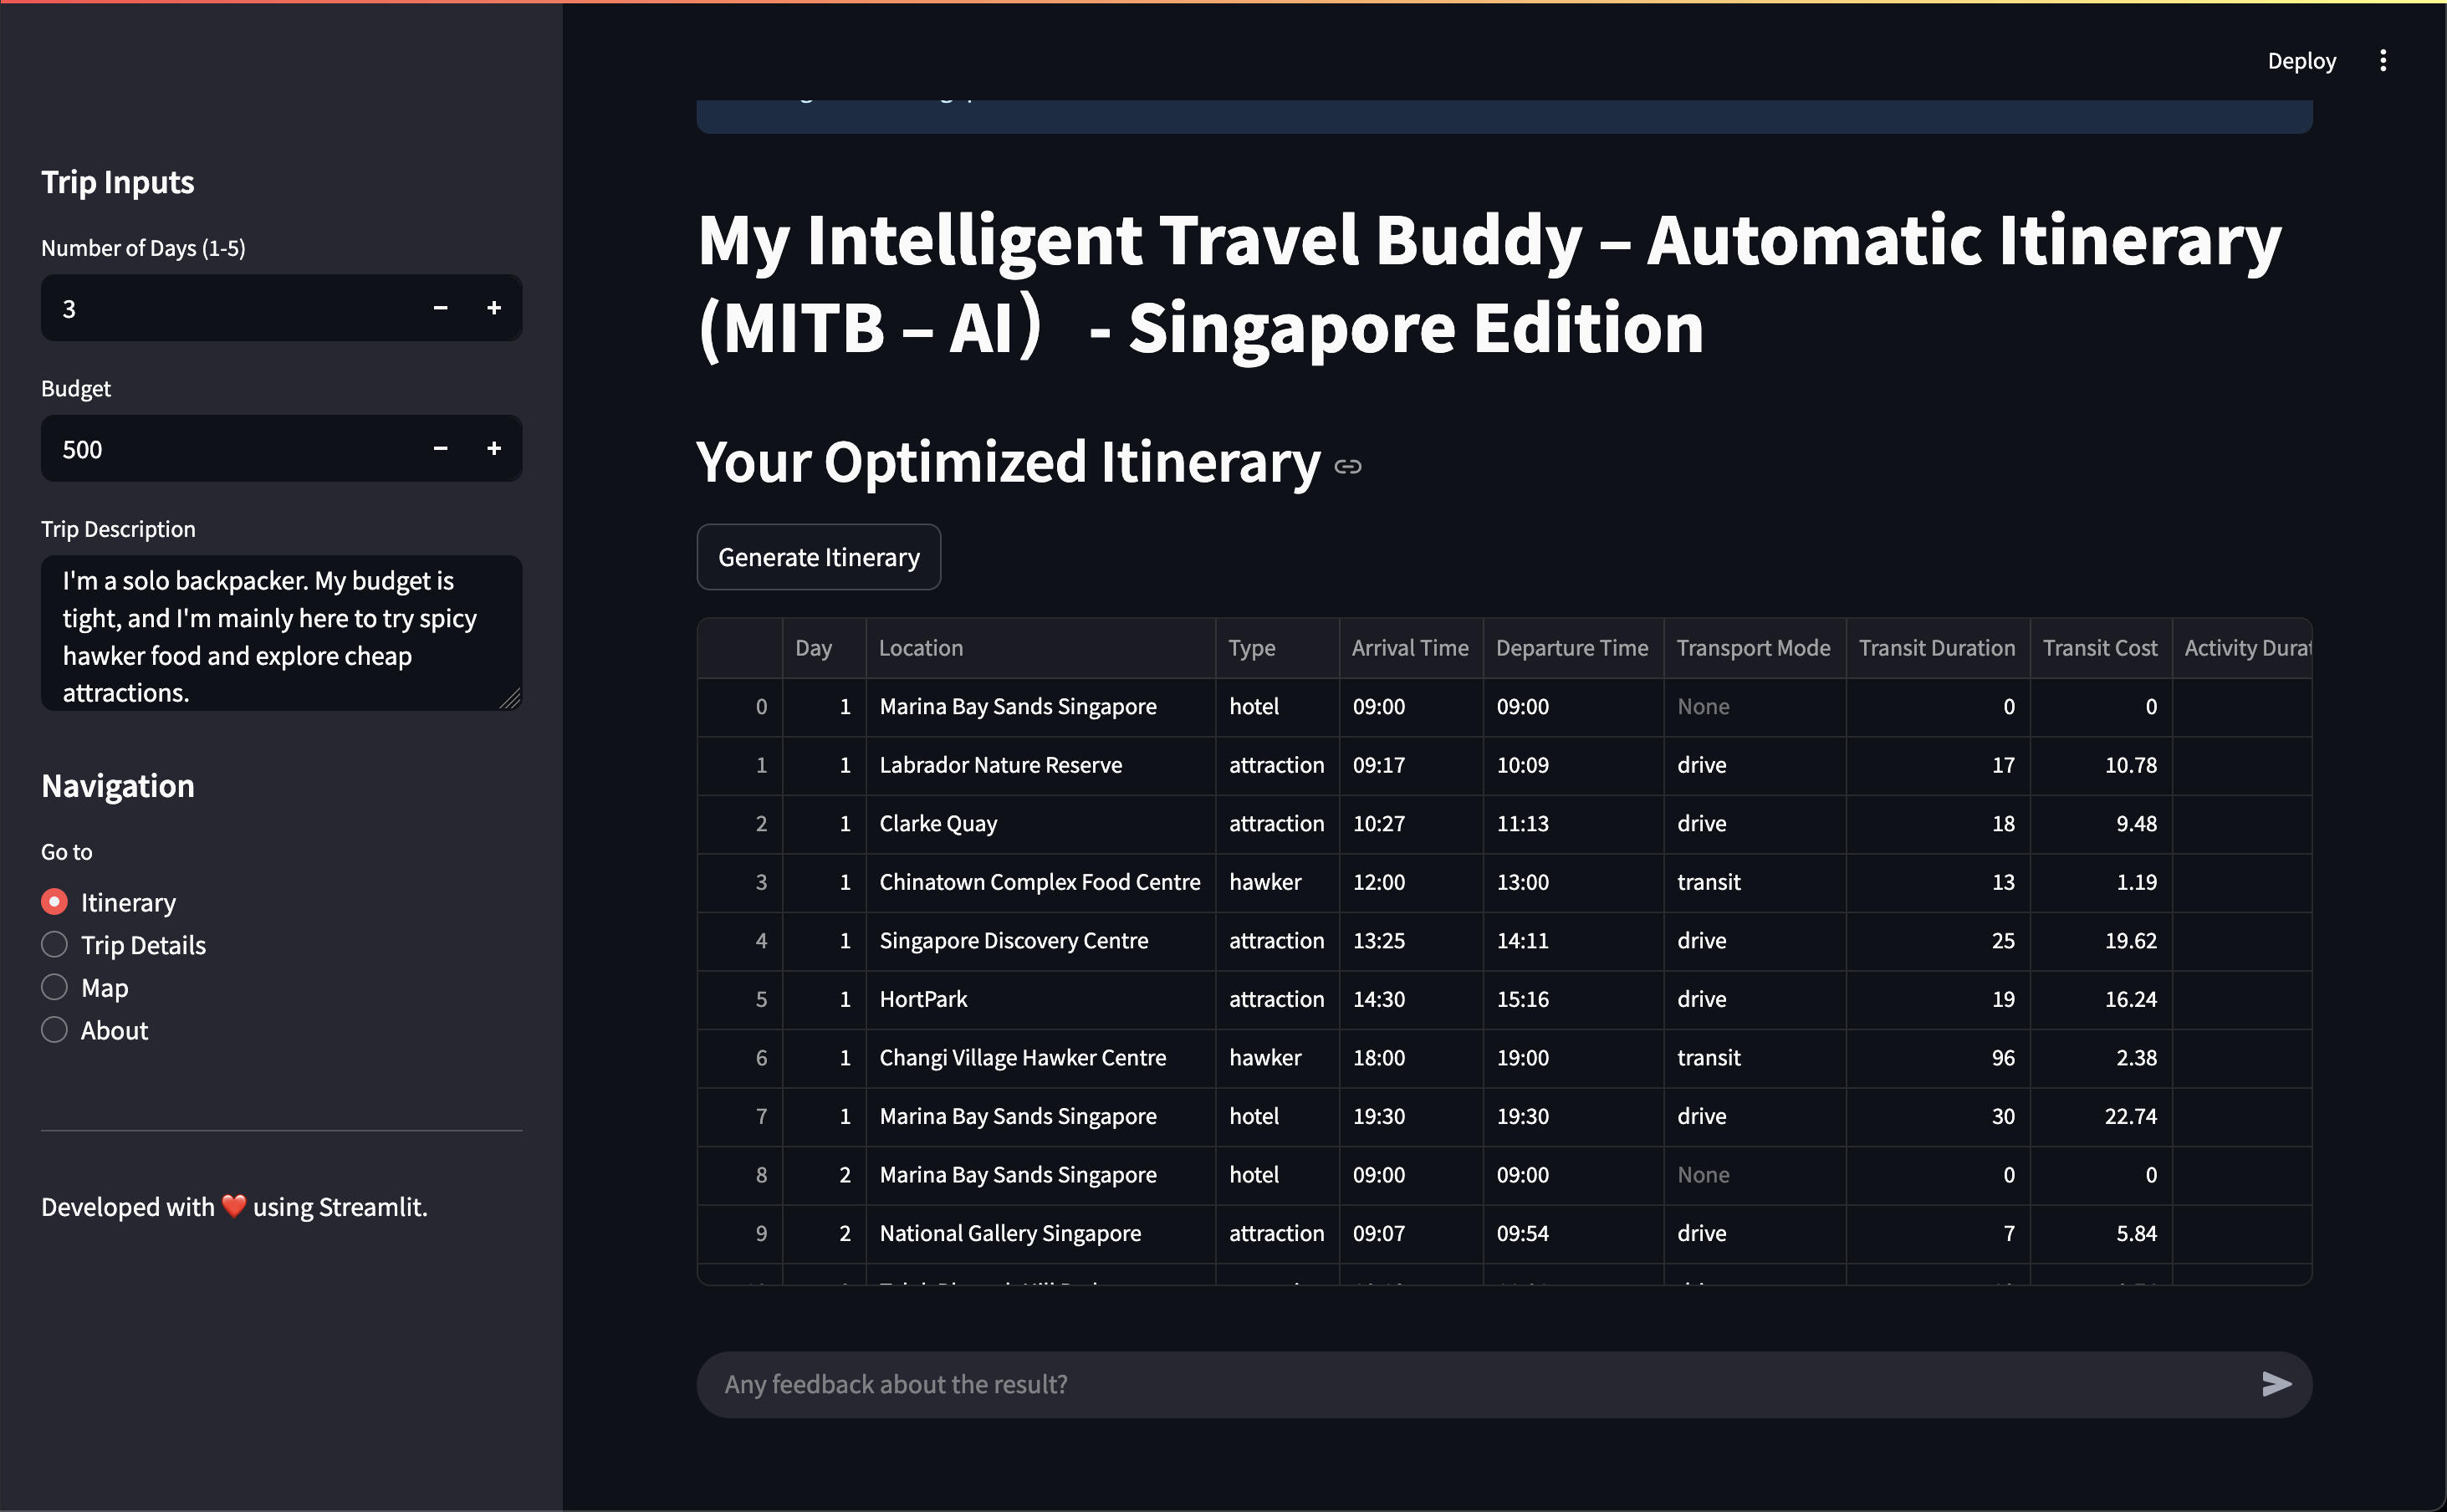
\includegraphics[width=0.75\linewidth]{user_interface.png}
    \caption{Basic User Interface for Itinerary Planning}
    \label{fig:enter-label}
\end{figure}
\vspace{-0.2cm}

Here is the example itinerary when the user stated profile of:
\begin{itemize}
    \item Number of days: 3
    \item Budget: 300 SGD
    \item Trip Description: "I'm a solo backpacker. My budget is tight, and I'm mainly here to try spicy food and explore cheap attractions."
\end{itemize}

\begin{figure}[H]
    \centering
    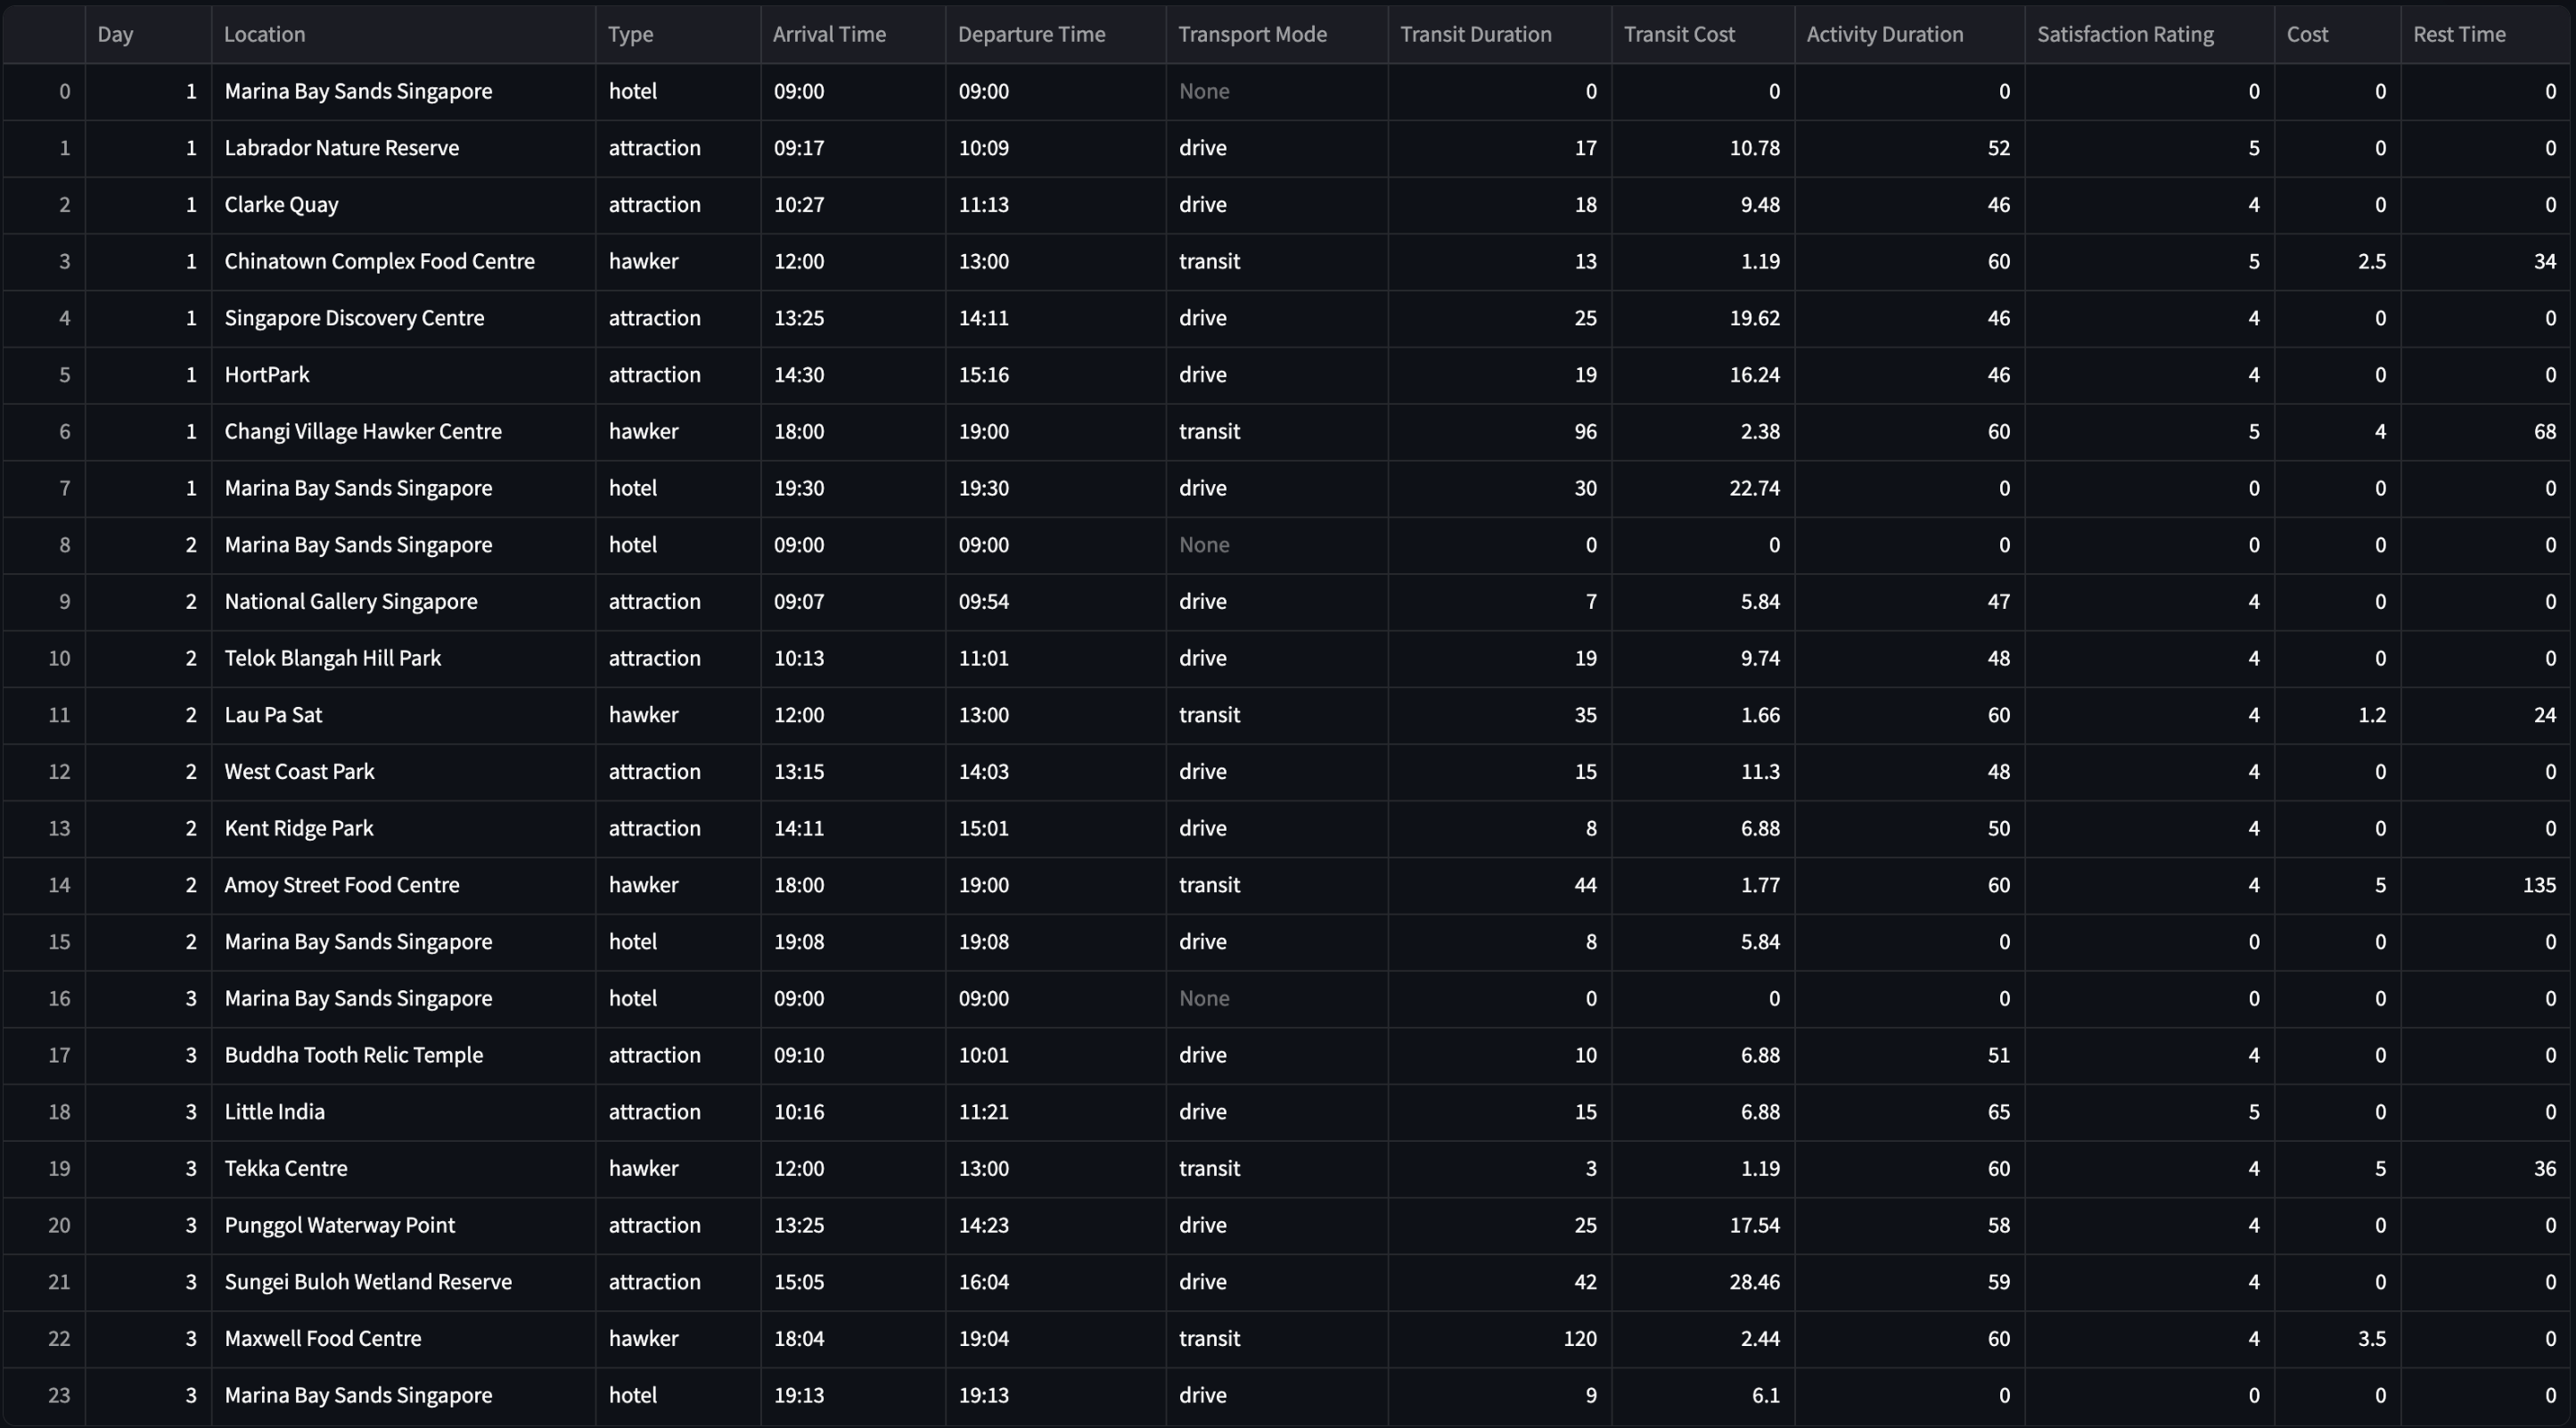
\includegraphics[width=0.75\linewidth]{itinerary_initial.png}
    \caption{Initial Itinerary for solo backpacker}
    \label{fig:enter-label}
\end{figure}
\vspace{-0.2cm}

The user is able to ask the LLM to modify the itinerary if there are any change of plans or something similar.
\vspace{-0.2cm}

\begin{figure}[H]
    \centering
    
\includegraphics[width=0.75\linewidth]{feedback_prompt.png}
    \caption{Feedback prompt from the user}
    \label{fig:enter-label}
\end{figure}
\vspace{-0.4cm}

\begin{figure}[H]
    \centering
    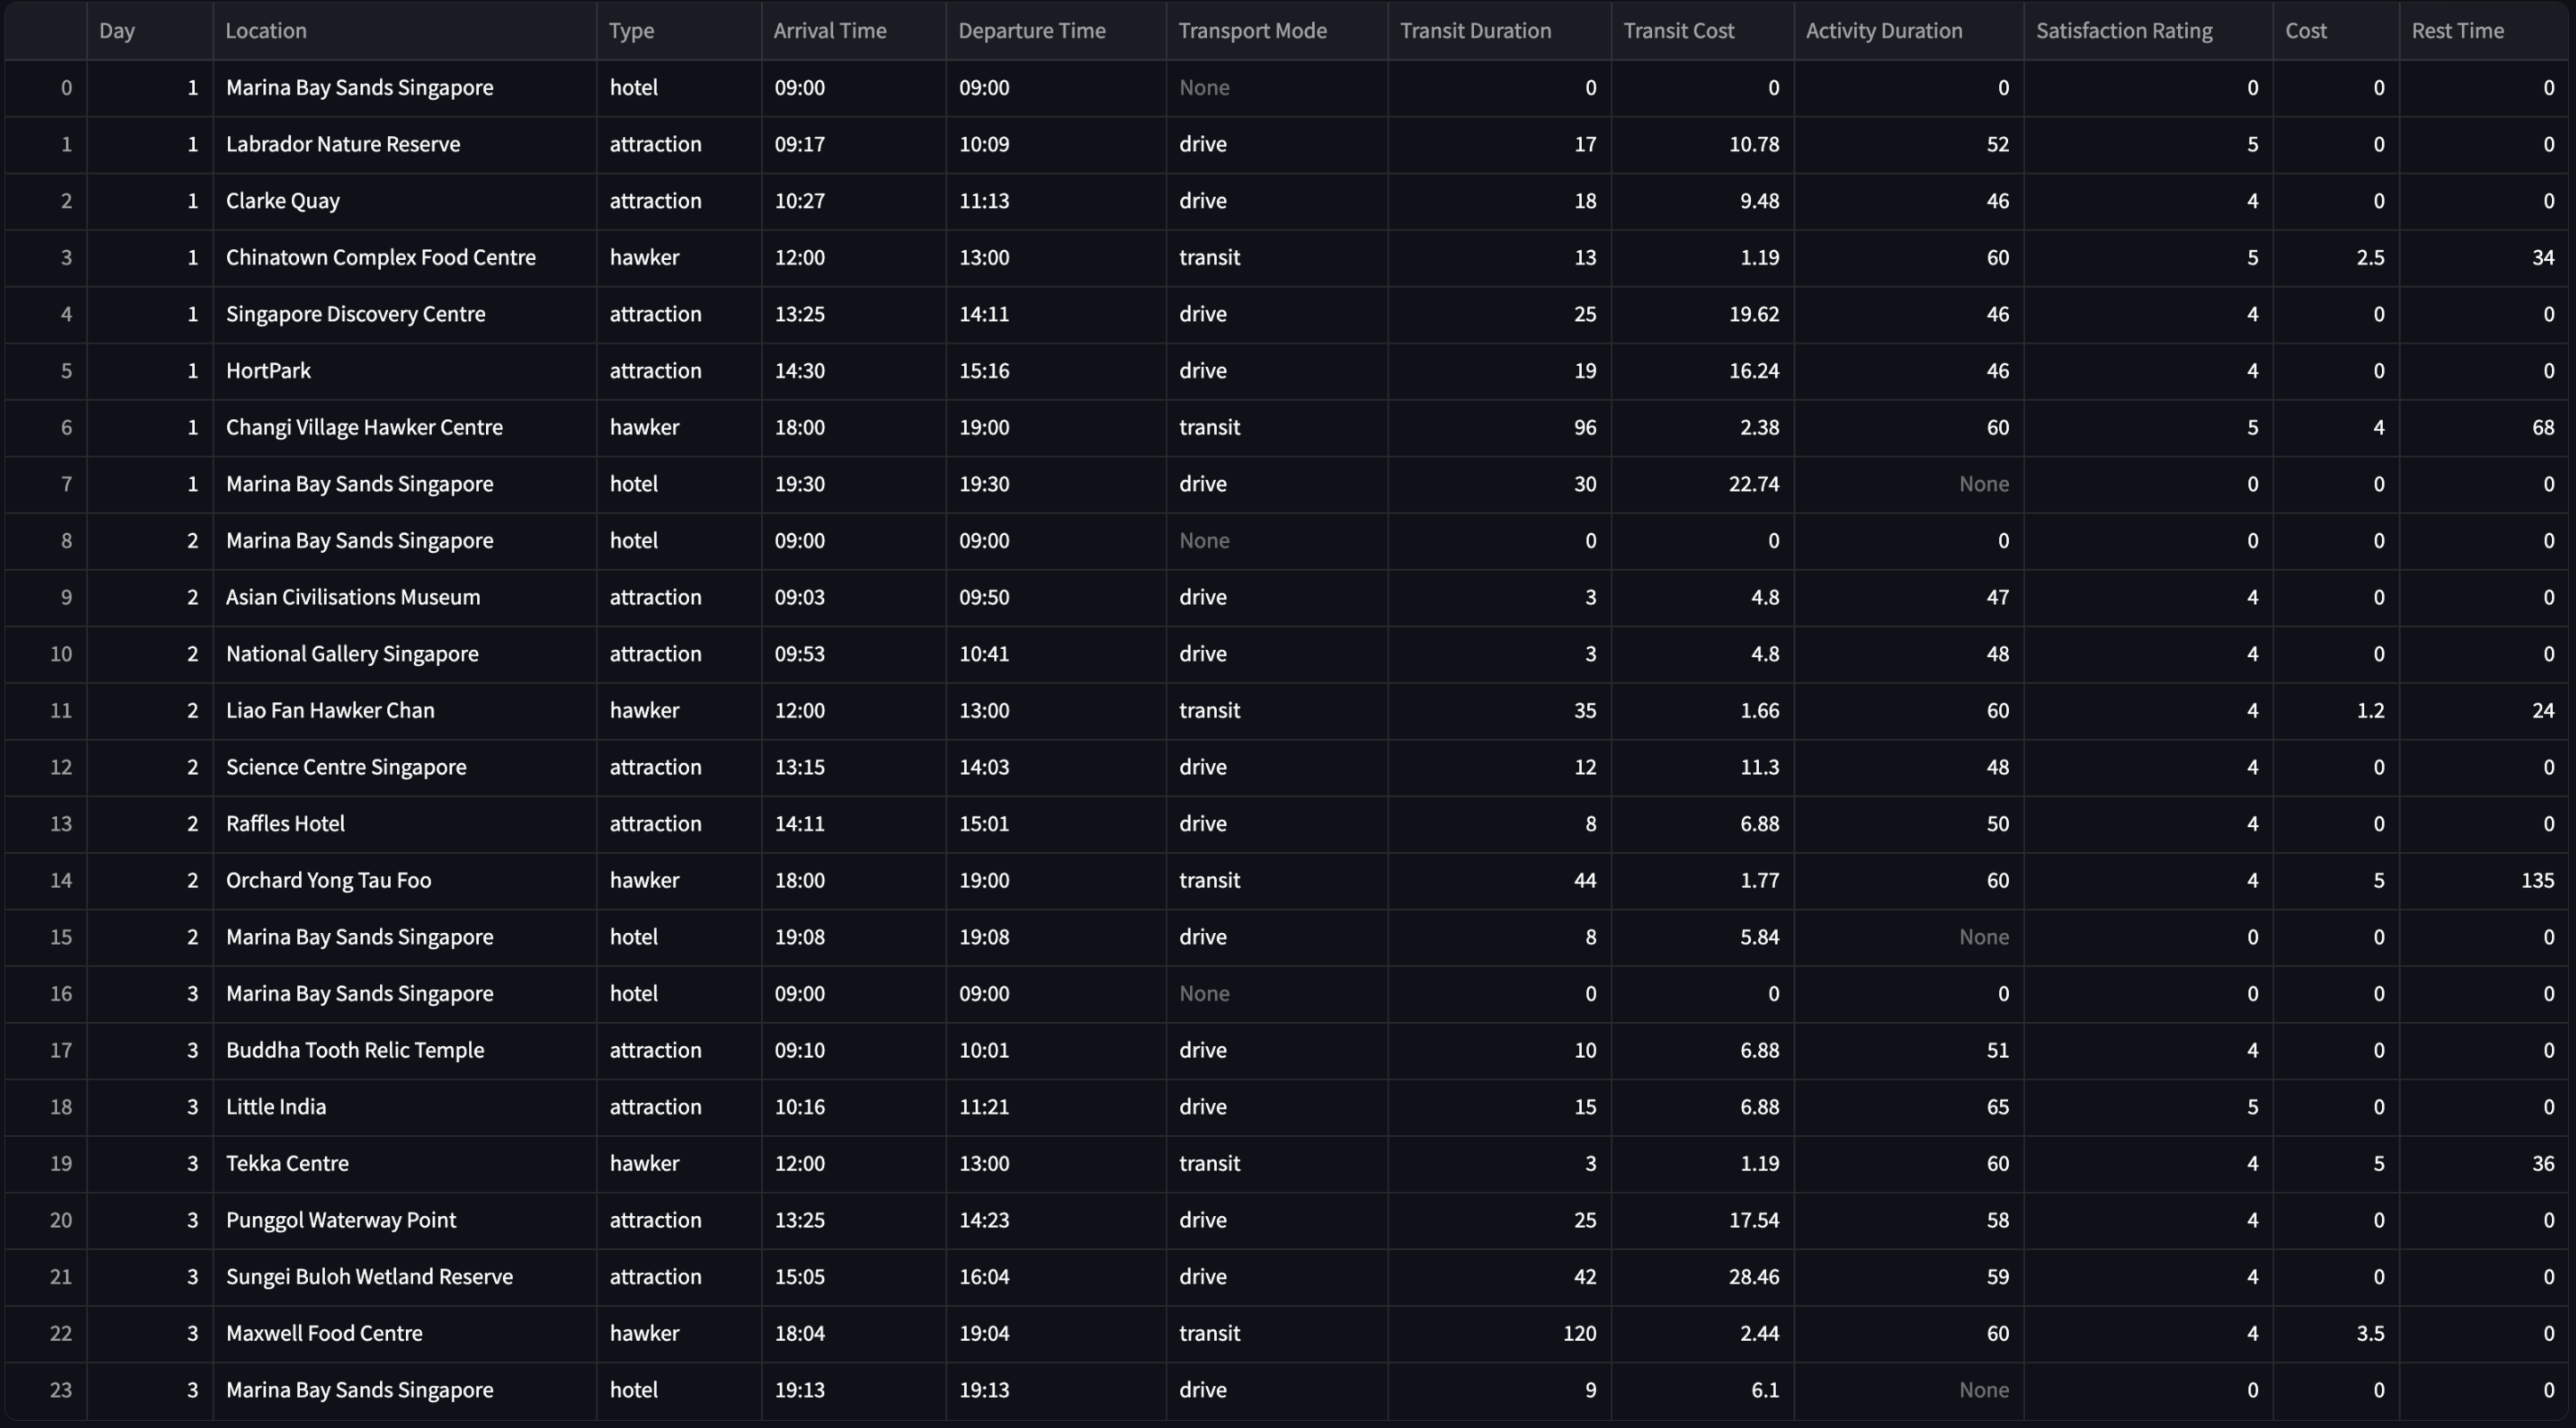
\includegraphics[width=0.75\linewidth]{itinerary_modified.png}
    \caption{Modified Itinerary for solo backpacker}
    \label{fig:enter-label}
\end{figure}

Itinerary was modified as the user requested a change in 2nd-day plan to cater for wet-weather due to the weather forecast. Outdoor attractions in the initial itinerary (e.g. West Coast Park, Kent Ridge Park) are replaced with indoor ones (e.g. Science Centre Singapore, Raffles Hotel).

\section{Conclusion and Future Work}
MITB-AI demontrates the feasibility and benefits of combining LLMs with optimization algorithms for travel itinerary generation. By decomposing the planning task across a multi-agent LLM framework and integrating ALNS for itinerary scheduling, the system offers a scalable, customizable, and context-aware solution. Our work highlights how LLMs, when enhanced with memory, tool use, and structured reasoning capabilities, can go beyond language generation to support decision-making in constrained real-world domains.

Future enhancements to MITB-AI will focus on incorporating additional real-time constraints such as planning according to real-time transport events, weather forecasts, accessibility, and events affecting availability. We also plan to add more granularity to the problem set to make it more-realistic, for example multiple hotel options and different opening and closing time for different POIs. Moreover, expanding the system to support other cities will be a key step toward validating its generalizability and robustness. Integration with real booking systems, user authentication, and mobile interfaces will also be explored as we move toward actual deployment to users. 

% For instructions on how to submit your work to ECAI and on matters such 
% as page limits or referring to supplementary material, please consult 
% the Call for Papers of the next edition of the conference. Keep in mind
% that you must use the \texttt{doubleblind} option for submission. 

% You presumably are already familiar with the use of \LaTeX. But let 
% us still have a quick look at how to typeset a simple equation: 
% %
% \begin{eqnarray}\label{eq:vcg}
% p_i(\boldsymbol{\hat{v}}) & = &
% \sum_{j \neq i} \hat{v}_j(f(\boldsymbol{\hat{v}}_{-i})) - 
% \sum_{j \neq i} \hat{v}_j(f(\boldsymbol{\hat{v}})) 
% \end{eqnarray}
% %
% Use the usual combination of \verb|\label{}| and \verb|\ref{}| to 
% refer to numbered equations, such as Equation~(\ref{eq:vcg}). 
% Next, a theorem: 

% \begin{theorem}[Fermat, 1637]\label{thm:fermat}
% No triple $(a,b,c)$ of natural numbers satisfies the equation 
% $a^n + b^n = c^n$ for any natural number $n > 2$.
% \end{theorem}

% \begin{proof}
% A full proof can be found in the supplementary material.
% \end{proof}

% Table captions should be centred \emph{above} the table, while figure 
% captions should be centred \emph{below} the figure.\footnote{Footnotes
% should be placed \emph{after} punctuation marks (such as full stops).}
 
% \begin{table}[h]
% \caption{Locations of selected conference editions.}
% \centering
% \begin{tabular}{ll@{\hspace{8mm}}ll} 
% \toprule
% AISB-1980 & Amsterdam & ECAI-1990 & Stockholm \\
% ECAI-2000 & Berlin & ECAI-2010 & Lisbon \\
% ECAI-2020 & \multicolumn{3}{l}{Santiago de Compostela (online)} \\
% \bottomrule
% \end{tabular}
% \end{table}

%%%%%%%%%%%%%%%%%%%%%%%%%%%%%%%%%%%%%%%%%%%%%%%%%%%%%%%%%%%%%%%%%%%%%%%%


%%% Use this command to include your bibliography file.

\bibliography{mybibfile}
\begin{enumerate}
    \item Barua, B., \& Kaiser, M. (2024). Optimizing Travel Itineraries with AI Algorithms in a Microservices Architecture: Balancing Cost, Time, Preferences, and Sustainability. Retrieved from https://arxiv.org/abs/2410.17943
    \item Fan, Z., Ghaddar, B., Wang, X., Xing, L., Zhang, Y., \& Zhou, Z. (2024, January 06). Artificial Intelligence for Operations Research: Revolutionizing the Operations Research Process. Retrieved from ARXIV: https://arxiv.org/html/2401.03244v1
    \item JP Morgan AI Research. (2024). TRIP-PAL: Travel Planning with Guarantees by Combining Large Language Models and Automated Planners. JP Morgan AI Research. Retrieved from https://arxiv.org/pdf/2406.10196
    \item Khamsing, K. L. (2021). Modified ALNS Algorithm for a Processing Application of Family Tourist Route Planning: A Case Study of Buriram in Thailand. Mathematics, 9(2). doi:https://doi.org/10.3390/math9020023
    \item Pelago. (2025). Pelago - Get inspired for your next trip. Retrieved from Pelago by Singapore Airlines: https://www.pelago.com/en-SG/trip-planner/
\end{enumerate}

\end{document}
%%%%%%%%%%%%%%%%%%%%%%%%%%%%%%%%%%%%%%%%%%%%%%%%%%%%%%%%%%%%%%%%%%%%%%

Sure, here are the key pointers and follow-ups from the meeting:

Initial site selection using community centroids:


Concern that naively selecting community centroids as candidate sites without considering competitor and allied stores may miss out on potentially better nearby locations.
Suggestion to shift centroids away from competitors and towards population concentrations for better capture.
Explore metrics like silhouette index that consider cohesion to population and separation from competitors.


Varying community granularity:


Instead of fixing community sizes, explore varying the granularity - make communities smaller or larger.
This allows searching a larger solution space and potentially finding better centroids/sites.
Relates to the idea of making the discrete approach tend towards a continuous solution space.


Two-level site selection:


First select top sites within each micro-community/smaller granularity.
Then combine these top micro-sites as candidates for the overall macro-community selection.


Comparison with continuous approach:


A major contribution could be showing the discrete community approach performs comparably to a continuous approach, but with much higher computational efficiency.
This requires implementing and comparing against a true continuous baseline.


Clarify terminology:


Need to clearly define and distinguish between "solution neighborhood", "search space", etc. in the paper.
Response required to the reviewer's comment seeking clarification on these terms.


Rework/strengthen contributions:


Some concerns that the stated contributions (discrete to continuous, eliminating human bias, generalizability) may not be very strong.
Need to rethink and articulate the real novel contributions more convincingly.


Literature review:


Review recent literature to identify relevant work still using static/non-dynamic models to better justify this approach.


Meeting with Proflow:


Proflow wants to see the full paper draft before the next meeting, likely early next week.
Kar Way may not be available tomorrow due to his daughter's school event.

Overall, there are suggestions to improve the site selection process, explore varying granularities, compare against a continuous baseline, clarify terminology, rework the contributions, review recent literature, and prepare for the next meeting with the full draft.
